\documentclass[b4paper, landscape, dvipdfmx]{jsarticle}
%----- 必要なパッケージ -----
\usepackage{fancybox,ascmac,otf,ulem}
\usepackage{amssymb, amsthm}
\usepackage[leqno]{amsmath}
\usepackage{geometry}
\usepackage{multicol}
\usepackage{tcolorbox}
\usepackage{xcolor}
\usepackage{fancyhdr}
\usepackage{tikz}

% shadowsライブラリ
\usetikzlibrary{
    positioning,
    arrows.meta,
    calc,
    shadows,
    shadows.blur,
    intersections
}

\tcbuselibrary{skins, breakable, theorems}
\usepackage{enumitem}
\setlist[enumerate,1]{label=(\arabic*)}
\setlist[itemize]{leftmargin=*}
\newcommand{\ds}{\displaystyle}

%----- レイアウト設定 -----
\geometry{
  left=15mm,
  right=15mm,
  top=20mm,
  bottom=15mm,
  headheight=25pt
}

%----- 数式環境の上下の余白調整 -----
\AtBeginDocument{
  \setlength{\abovedisplayskip}{5pt}
  \setlength{\belowdisplayskip}{5pt}
  \setlength{\abovedisplayshortskip}{0pt}
  \setlength{\belowdisplayshortskip}{3pt}
}

%===========================================================
%  デザイン設定
%===========================================================

%--- 色の定義 ---
\definecolor{printBlue}{RGB}{0, 50, 100}     % 濃紺
\definecolor{printRed}{RGB}{140, 20, 20}     % 濃エンジ
\definecolor{printTeal}{RGB}{0, 60, 60}      % 濃い青緑

%--- 共通スタイル定義 ---
\tcbset{
    chartbox/.style={
        enhanced,
        fonttitle=\sffamily\bfseries,
        boxrule=1pt,
        arc=2pt,
        top=1.0em,
        nobeforeafter,
        enlarge left by=-2mm,
        enlarge right by=-2mm,
        drop fuzzy shadow,
        colback=white,
        attach boxed title to top left={xshift=10pt, yshift*=-\tcboxedtitleheight/2},
        boxed title style={frame hidden, sharp corners, rounded corners=southeast, arc=3pt}
    }
}

% 各種ボックス環境定義
\newtcolorbox{any}[1]{
    enlarge left by=0mm, enlarge right by=0mm,
    enhanced, frame hidden, colback=white, title={#1},
    attach boxed title to top left={xshift=0mm, yshift=0mm},
    coltitle=white, fonttitle=\bfseries\sffamily,
    boxed title style={
        colback=black!80, frame hidden, arc=4pt, outer arc=4pt,
        sharp corners=south, boxrule=0pt,
        top=1mm, bottom=1mm, left=3mm, right=3mm
    },
    underlay boxed title={
        \draw[thick, black!80] (title.south west) -- (title.south west-|frame.east);
    },
    breakable, top=5mm, left=2mm, right=2mm, bottom=0mm,
    before skip=1em, after skip=1em,
    segmentation style={draw=black!40, dashed}
}

\newenvironment{eg}[1]{
\begin{tcolorbox}[
    chartbox,
    colframe=printBlue,
    coltitle=white,
    title=\textbf{例題 #1},
    boxed title style={colback=printBlue},
    segmentation style={draw=printBlue, line width=0.5pt, dashed}
]}
{\end{tcolorbox}}

\newenvironment{prac}[1]{
\begin{tcolorbox}[
    chartbox,
    colframe=printRed,
    coltitle=white,
    title=\textbf{練習 #1},
    boxed title style={colback=printRed}
]}
{\end{tcolorbox}}

\newenvironment{thm}[1]{
\begin{tcolorbox}[
    chartbox,
    colframe=printTeal,
    coltitle=white,
    title=\textbf{#1},
    boxed title style={colback=printTeal}
]}
{\end{tcolorbox}}

% インデント修正済み answer 環境
\newenvironment{answer}[1][height fill]{
    \begin{tcolorbox}[
        enhanced,
        title={Memo / Answer},
        colframe=black!80,
        colback=white,
        coltitle=black!60,
        fonttitle=\sffamily\bfseries,
        attach boxed title to top left={xshift=5mm, yshift*=-\tcboxedtitleheight/2},
        boxed title style={frame hidden, colback=white},
        boxrule=1pt,
        arc=1pt,
        nobeforeafter,
        enlarge left by=-2mm, 
        enlarge right by=-2mm, 
        height fill,
        segmentation style={draw=black!20, solid},
        underlay={
            \begin{tcbclipinterior}
                \draw[step=5mm, black!5, ultra thin] (interior.south west) grid (interior.north east);
            \end{tcbclipinterior}
        }, 
        #1
    ]}
{ \end{tcolorbox}}

%----- 段組の設定 -----
\setlength{\columnsep}{15mm}
\setlength{\columnseprule}{0.4pt}
\renewcommand{\columnseprulecolor}{\color{black!30}}

%----- ヘッダーの設定 -----
\pagestyle{fancy}
\fancyhf{}

% ヘッダーデザイン
\fancyhead[C]{%
    \begin{tikzpicture}[remember picture, overlay]
        \node[anchor=north west, fill=printBlue, minimum width=\paperwidth, minimum height=5pt] at (current page.north west) {};
    \end{tikzpicture}
}
\fancyhead[L]{\small \textcolor{black!90}{数学C $>$ 第1章--平面ベクトル $>$ 第1回--\textbf{ベクトルの定義と演算}}}
\fancyhead[R]{\small 年 \hspace{1cm} 組 \hspace{1cm} 番 \quad 氏名 \hspace{6cm}}
\renewcommand{\headrulewidth}{0pt}

\begin{document}

%=============================================================================
% 1枚目:定義と和・差(基本概念)
%=============================================================================
\begin{multicols}{2}

%-----------------------------------------------------------------------------
% 左カラム:ベクトルの本質と定義
%-----------------------------------------------------------------------------
\begin{any}{1. ベクトルとは何か}
    \begin{itemize}
        \item \textbf{スカラー (scalar)}: 大きさだけで決まる量(例:長さ, 質量, 温度, エネルギー).
        \item \textbf{ベクトル (vector)}: \textbf{「大きさ」}と\textbf{「向き」}を持つ量(例:速度, 力, 変位).
    \end{itemize}

    ベクトルは図形的には「有向線分」として表されるが, 本質的には「点Aを点Bに移す\textbf{平行移動}」を表す量である.

    \begin{thm}{用語と定義}
    \begin{enumerate}
        \item \textbf{表記}: 始点A, 終点Bのベクトルを $\overrightarrow{\text{AB}}$ と書く. 1文字で $\vec{a}$ とも書く.
        \item \textbf{大きさ}: 線分の長さ. $|\vec{a}|$ または $|\overrightarrow{\text{AB}}|$ と書く.
        \item \textbf{ベクトルの相等}: 「向き」と「大きさ」が同じならば, 始点がどこにあっても\textbf{同じベクトル}とみなす.
        \[ \vec{a} = \vec{b} \]
        \item \textbf{逆ベクトル}: 大きさが同じで向きが反対のベクトル. $\vec{a}$ に対し $-\vec{a}$ と書く.
        \item \textbf{ゼロベクトル}: 大きさが0のベクトル $\vec{0}$. 向きは考えない. 始点と終点が一致する(移動しない).
    \end{enumerate}
    \begin{center}
    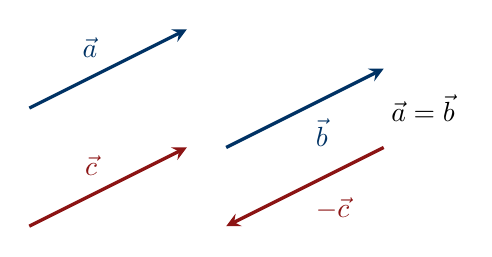
\begin{tikzpicture}[scale=1.0, >=stealth]
        % Equal vectors
        \draw[->, very thick, printBlue] (0,0) -- (2,1) node[midway, above left] {$\vec{a}$};
        \draw[->, very thick, printBlue] (2.5,-0.5) -- (4.5,0.5) node[midway, below right] {$\vec{b}$};
        \node at (5, 0) {$\vec{a} = \vec{b}$};
        
        % Inverse vector
        \draw[->, very thick, printRed] (0,-1.5) -- (2,-0.5) node[midway, above left] {$\vec{c}$};
        \draw[->, very thick, printRed] (4.5,-0.5) -- (2.5,-1.5) node[midway, below right] {$-\vec{c}$};
    \end{tikzpicture}
    \end{center}
     \end{thm}
\end{any}

%-----------------------------------------------------------------------------
% 右カラム:和と差の定義
%-----------------------------------------------------------------------------
\columnbreak

\begin{any}{2. ベクトルの和と差}
    ベクトルの演算は「物理的な継ぎ足し」として定義される.

    \begin{thm}{和の定義(三角形の法則・平行四辺形の法則)}
        $\vec{a}$ 進んでから $\vec{b}$ 進むことは, $\vec{a}+\vec{b}$ 進むことに等しい.
        \[ \overrightarrow{\text{AB}} + \overrightarrow{\text{BC}} = \overrightarrow{\text{AC}} \]
        
        \vspace{0.5em}
        \centering
        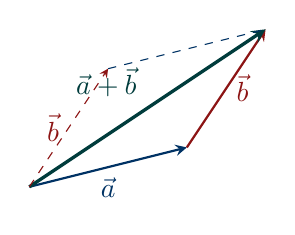
\begin{tikzpicture}[scale=1, >=stealth]
            \coordinate (A) at (0,0);
            \coordinate (B) at (2,0.5);
            \coordinate (C) at (3,2);
            \coordinate (D) at (1,1.5);
            
            % Triangle
            \draw[->, thick, printBlue] (A) -- (B) node[midway, below] {$\vec{a}$};
            \draw[->, thick, printRed] (B) -- (C) node[midway, right] {$\vec{b}$};
            \draw[->, very thick, printTeal] (A) -- (C) node[midway, above left] {$\vec{a}+\vec{b}$};
            
            % Parallelogram parts
            \draw[->, dashed, printRed] (A) -- (D) node[midway, left] {$\vec{b}$};
            \draw[dashed, printBlue] (D) -- (C);
        \end{tikzpicture}
    \end{thm}

    \begin{thm}{差の定義(逆ベクトルの和)}
        数の引き算 $5 - 3 = 5 + (-3)$ と同様に, ベクトルの差は\textbf{「逆ベクトルを足す」}こととして定義する.
        \[ \vec{a} - \vec{b} = \vec{a} + (-\vec{b}) \]
        
        \vspace{0.5em}
        \textbf{作図の手順:}
        \begin{enumerate}
            \item $\vec{a}$ を描く.
            \item $\vec{a}$ の終点に, $\vec{b}$ と逆向きのベクトル $-\vec{b}$ を継ぎ足す.
            \item 始点から最後の終点を結ぶ.
        \end{enumerate}
        
        \vspace{1em}
        \centering
        \begin{tikzpicture}[scale=1, >=stealth]
            \coordinate (Start) at (0,0);
            \coordinate (A) at (3,1);
            \coordinate (B_vec) at (1,1.5); % vector b relative
            
            % Draw a
            \draw[->, thick, printBlue] (Start) -- (A) node[midway, below right] {$\vec{a}$};
            
            % Draw -b from tip of a
            % -b is (-1, -1.5)
            \coordinate (End) at ($(A) - (B_vec)$);
            \draw[->, thick, printRed] (A) -- (End) node[midway, right] {$-\vec{b}$};
            
            % Result
            \draw[->, very thick, printTeal] (Start) -- (End) node[midway, below left] {$\vec{a}-\vec{b}$};
            
            % Reference: Show b somewhere else or dashed
            \draw[->, dashed, gray] (Start) -- ++(B_vec) node[midway, left] {$\vec{b}$};
            \node[gray, scale=0.8] at (0.5, 2.0) {(参考)};
        \end{tikzpicture}
    \end{thm}
    
    \begin{tcolorbox}[colback=yellow!10, frame hidden, title={重要:位置ベクトルの視点}]
        始点をOにそろえて考えると, 上図の結果は
        \[ \overrightarrow{\text{OA}} - \overrightarrow{\text{OB}} = \overrightarrow{\text{BA}} \quad (\text{引く方の終点} \to \text{引かれる方の終点}) \]
        となっている. 実戦ではこの「視点」で計算することが多い.
    \end{tcolorbox}
\end{any}

\end{multicols}

%=============================================================================
% 2枚目:実数倍・平行・分解
%=============================================================================
\newpage
\begin{multicols}{2}

%-----------------------------------------------------------------------------
% 左カラム:実数倍と平行
%-----------------------------------------------------------------------------
\begin{any}{3. 実数倍と平行条件}
    ベクトル $\vec{a}$ を $k$ 倍する($k$ は実数).
    \begin{itemize}
        \item 大きさは $|k|$ 倍になる. ($|k\vec{a}| = |k||\vec{a}|$)
        \item $k>0$ なら向きは同じ, $k<0$ なら向きは反対.
    \end{itemize}

    \begin{thm}{平行条件}
        $\vec{a} \neq \vec{0}, \vec{b} \neq \vec{0}$ のとき,
        \[ \vec{a} // \vec{b} \iff \vec{b} = k\vec{a} \quad (\text{$k$は実数}) \]
    \end{thm}
    
    \textbf{単位ベクトル:}
    大きさが $1$ のベクトルを単位ベクトルという. 
    $\vec{a}$ と同じ向きの単位ベクトル $\vec{e}$ は, $\vec{a}$ を自身の大きさで割ることで得られる.
    \[ \vec{e} = \frac{\vec{a}}{|\vec{a}|} \]
\end{any}

\begin{eg}{1 (計算規則)}
    通常の文字式と同様に計算できる. 次の等式を満たす $\vec{x}$ を求めよ.
    \[ 2(\vec{x} - 3\vec{a}) = \vec{x} + 4\vec{b} \]
    \tcblower
    \vspace{8cm}
\end{eg}

%-----------------------------------------------------------------------------
% 右カラム:ベクトルの分解(例題)
%-----------------------------------------------------------------------------
\columnbreak

\begin{any}{4. ベクトルの分解}
    平面上の任意のベクトルは, 平行でない2つのベクトル(基底)を用いてただ1通りに表すことができる.
    \textbf{「道順」}を辿るイメージで分解していく.

    \begin{eg}{2 (正六角形と分解)}
        正六角形ABCDEFにおいて, $\overrightarrow{\text{AB}}=\vec{a}, \overrightarrow{\text{AF}}=\vec{b}$ とする.
        次のベクトルを $\vec{a}, \vec{b}$ を用いて表せ.
        \begin{enumerate}
            \item $\overrightarrow{\text{AO}}$
            \item $\overrightarrow{\text{AC}}$
            \item $\overrightarrow{\text{BD}}$
        \end{enumerate}
        
        \begin{center}
        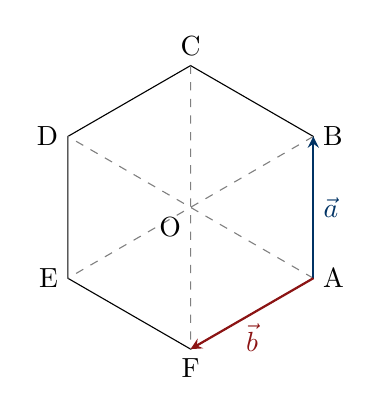
\begin{tikzpicture}[scale=1.2, >=stealth]
            \coordinate (O) at (0,0);
            \coordinate (A) at (-30:1.5);
            \coordinate (B) at (30:1.5);
            \coordinate (C) at (90:1.5);
            \coordinate (D) at (150:1.5);
            \coordinate (E) at (210:1.5);
            \coordinate (F) at (270:1.5);

            \draw (A)--(B)--(C)--(D)--(E)--(F)--cycle;
            \draw[dashed, gray] (A)--(D) (B)--(E) (C)--(F);
            
            \node[right] at (A) {A}; \node[right] at (B) {B}; \node[above] at (C) {C};
            \node[left] at (D) {D}; \node[left] at (E) {E}; \node[below] at (F) {F};
            \node[below left] at (O) {O};

            \draw[->, thick, printBlue] (A) -- (B) node[midway, right] {$\vec{a}$};
            \draw[->, thick, printRed] (A) -- (F) node[midway, below] {$\vec{b}$};
        \end{tikzpicture}
        \end{center}
        \tcblower
        \vspace{8cm}
    \end{eg}
\end{any}

\end{multicols}

%=============================================================================
% 3枚目:確認テスト(問題)
%=============================================================================
\newpage
\fancyhead[L]{\small \textcolor{black!90}{数学C $>$ 第1章--平面ベクトル $>$ 第1回--\textbf{確認テスト}}}
\begin{multicols}{2}

\begin{any}{確認テスト (A: 基本)}
    \begin{prac}{A1 (作図)}
        右の図を利用して, 以下のベクトルを作図せよ.
        \begin{enumerate}
            \item $\vec{a} + \vec{b}$
            \item $\vec{a} - \vec{b}$ \quad ($\vec{a}$ に $-\vec{b}$ を足す)
        \end{enumerate}
        \vspace{1em}
        \begin{center}
        \begin{tikzpicture}[scale=0.8, >=stealth]
            \draw[step=1, gray!30, very thin] (-0.5,-2.5) grid (5.5, 2.5);
            \coordinate (O) at (2,0);
            \coordinate (A) at (4,1); % vec a = (2,1)
            \coordinate (B) at (3,-1); % vec b = (1,-1)
            
            \draw[->, thick, printBlue] (O) -- (A) node[midway, above left] {$\vec{a}$};
            \draw[->, thick, printRed] (O) -- (B) node[midway, below left] {$\vec{b}$};
            \fill[gray!50] (O) circle (2pt) node[left] {始点};
        \end{tikzpicture}
        \end{center}
    \end{prac}

    \begin{prac}{A2 (計算)}
        次の等式を満たす $\vec{x}$ を $\vec{a}, \vec{b}$ で表せ.
        \[ 3(\vec{x} - 2\vec{a}) + 2(\vec{a} - 2\vec{x}) = 6\vec{b} \]
    \end{prac}

    \begin{answer}[height=8cm]
    \end{answer}
\end{any}

\columnbreak

\begin{any}{確認テスト (B: 標準)}
    \begin{prac}{B1 (正六角形)}
        正六角形ABCDEFにおいて, $\overrightarrow{\text{AB}}=\vec{a}, \overrightarrow{\text{BC}}=\vec{b}$ とする.
        次のベクトルを $\vec{a}, \vec{b}$ を用いて表せ.
        \begin{enumerate}
            \item $\overrightarrow{\text{AF}}$
            \item $\overrightarrow{\text{AD}}$
            \item $\overrightarrow{\text{CE}}$
        \end{enumerate}
        
        \begin{center}
        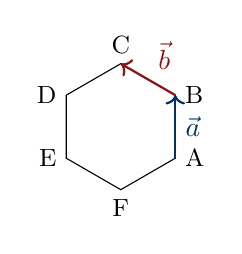
\begin{tikzpicture}[scale=0.8]
            \coordinate (A) at (-30:1.0);
            \coordinate (B) at (30:1.0);
            \coordinate (C) at (90:1.0);
            \coordinate (D) at (150:1.0);
            \coordinate (E) at (210:1.0);
            \coordinate (F) at (270:1.0);
            \draw (A)--(B)--(C)--(D)--(E)--(F)--cycle;
            \node[right] at (A) {\small A};
            \node[right] at (B) {\small B};
            \node[above] at (C) {\small C};
            \node[left] at (D) {\small D};
            \node[left] at (E) {\small E};
            \node[below] at (F) {\small F};
            \draw[->, thick, printBlue] (A)--(B) node[midway, right] {$\vec{a}$};
            \draw[->, thick, printRed] (B)--(C) node[midway, above right] {$\vec{b}$};
        \end{tikzpicture}
        \end{center}
    \end{prac}

    \begin{answer}[height=10cm]
    \end{answer}
\end{any}

\end{multicols}

%=============================================================================
% 4枚目:確認テスト(解答)
%=============================================================================
\newpage
\fancyhead[L]{\small \textcolor{black!90}{数学C $>$ 第1章--平面ベクトル $>$ 第1回 \textbf{【解答解説】}}}

\begin{multicols}{2}

\begin{any}{解答 (A: 基本)}
    \begin{prac}{A1 (作図)}
        (1) 平行四辺形の対角線. \\
        (2) $\vec{a}$ の終点から $\vec{b}$ と逆向きに進む.
        \vspace{1em}
        \begin{center}
        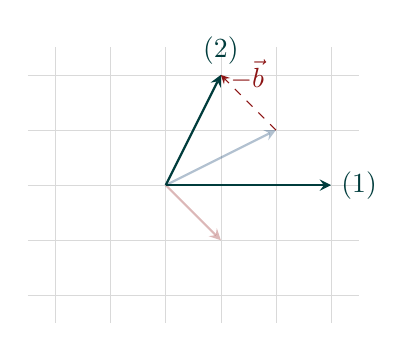
\begin{tikzpicture}[scale=0.7, >=stealth]
            \draw[step=1, gray!30, very thin] (-0.5,-2.5) grid (5.5, 2.5);
            \coordinate (O) at (2,0);
            \coordinate (A) at (4,1); 
            \coordinate (B) at (3,-1);
            
            \draw[->, thick, printBlue, opacity=0.3] (O) -- (A);
            \draw[->, thick, printRed, opacity=0.3] (O) -- (B);
            
            % Answer (1) a+b = (3,0)
            \draw[->, thick, printTeal] (O) -- (5,0) node[right] {(1)};
            
            % Answer (2) a-b = a + (-b). 
            % a is (2,1). -b is (-1,1). sum is (1,2).
            \draw[->, dashed, printRed] (A) -- (3,2) node[right] {$-\vec{b}$};
            \draw[->, thick, printTeal] (O) -- (3,2) node[above] {(2)};
        \end{tikzpicture}
        \end{center}
    \end{prac}

    \begin{answer}[height=8cm]
    \color{printRed}
    \textbf{A2 解答:} \\
    \begin{align*}
        3\vec{x} - 6\vec{a} + 2\vec{a} - 4\vec{x} &= 6\vec{b} \\
        -\vec{x} - 4\vec{a} &= 6\vec{b} \\
        -\vec{x} &= 4\vec{a} + 6\vec{b} \\
        \therefore \quad \vec{x} &= -4\vec{a} - 6\vec{b}
    \end{align*}
    \end{answer}
\end{any}

\columnbreak

\begin{any}{解答 (B: 標準)}
    \begin{answer}[height fill]
    \color{printRed}
    \textbf{B1 解答:} \\
    与えられた基底は $\overrightarrow{\text{AB}}=\vec{a}, \overrightarrow{\text{BC}}=\vec{b}$.
    
    (1) $\overrightarrow{\text{AF}}$ \\
    $\overrightarrow{\text{AF}}$ は $\overrightarrow{\text{CD}}$ と平行で逆向きだが, $\overrightarrow{\text{CD}} = \overrightarrow{\text{BA}} - \overrightarrow{\text{BC}}$ ? 複雑になる.\\
    正六角形の中心をOとすると, $\triangle ABO, \triangle BCO$ は正三角形. \\
    $\overrightarrow{\text{AO}} = \overrightarrow{\text{AB}} + \overrightarrow{\text{BO}} = \vec{a} + \vec{b}$. \\
    また $\overrightarrow{\text{AF}} = \overrightarrow{\text{BO}} - \overrightarrow{\text{BA}}$ の関係から...\\
    \textbf{最短ルート:} $\overrightarrow{\text{CD}} = \vec{b} - \vec{a}$ (前回参照).
    $\overrightarrow{\text{AF}}$ は $\overrightarrow{\text{CD}}$ の逆ベクトルである.
    \[ \overrightarrow{\text{AF}} = -\overrightarrow{\text{CD}} = -(\vec{b}-\vec{a}) = \boldsymbol{\vec{a} - \vec{b}} \]
    
    (2) $\overrightarrow{\text{AD}}$ \\
    ADはBCと平行で長さが2倍である.
    \[ \overrightarrow{\text{AD}} = 2\overrightarrow{\text{BC}} = \boldsymbol{2\vec{b}} \]
    
    (3) $\overrightarrow{\text{CE}}$ \\
    $\overrightarrow{\text{CE}} = \overrightarrow{\text{AE}} - \overrightarrow{\text{AC}}$. 
    まず $\overrightarrow{\text{AC}} = \vec{a} + \vec{b}$. \\
    $\overrightarrow{\text{AE}} = \overrightarrow{\text{AD}} + \overrightarrow{\text{DE}}$.
    $\overrightarrow{\text{DE}} = \overrightarrow{\text{BA}} = -\vec{a}$.
    よって $\overrightarrow{\text{AE}} = 2\vec{b} - \vec{a}$. \\
    したがって,
    \begin{align*}
        \overrightarrow{\text{CE}} &= (2\vec{b} - \vec{a}) - (\vec{a} + \vec{b}) \\
        &= \boldsymbol{\vec{b} - 2\vec{a}}
    \end{align*}
    
    \textbf{別解(図形的直観):}
    CEはBFと平行かつ等しい. $\overrightarrow{\text{BF}} = \overrightarrow{\text{AF}} - \overrightarrow{\text{AB}} = (\vec{a}-\vec{b}) - \vec{a} = -\vec{b}$ ...?
    図を確認すると, BFは $y$ 軸方向逆. $\overrightarrow{\text{AB}}=\vec{a}$ ($30^\circ$方向), $\overrightarrow{\text{BC}}=\vec{b}$ ($90^\circ$方向). 
    この組み合わせは少し難しい. 式変形で確実に解くのが良い.
    \end{answer}
\end{any}

\end{multicols}
\end{document}